A neural network is a class of mathematical function which uses non-linearities in order to increase representational power as compared to simple linear models.  They differ from other non-linear models like logistic regression by having multiple ``layers'' of nonlinearity between the input and the output.  These non-linearities are called \textit{activation functions}.  The multilayer perceptron is a simple example of neural network which is covered in the following section.

\subsection{Multilayer Perceptron}
A multilayer perceptron is a function $f:\mathbb{R}^n\rightarrow \mathbb{R}^m$. Given some vector $x\in \mathbb{R}^n$ of inputs, the output vector $f(x)\in\mathbb{R}^m$ of a multilayer perceptron is given by equation \ref{eq:mlp}
\begin{align}\label{eq:mlp}
    f(x) = \vec{\sigma_p} \circ T_p \circ\cdots\circ \vec{\sigma_2}\circ T_2\circ \vec{\sigma_1} \circ T_1\circ x
\end{align}
The functions $T_1,\dots,T_p$ are assumed to be affine and often represented as matrix multiplications plus constants.  The functions $\vec{\sigma_1},\dots,\vec{\sigma_p}$ are assumed to be nonlinear, each of these is an activation function.  In order for equation \ref{eq:mlp} to make sense, one must assume that the dimensions of each function are compatible with one another.  Activation functions are usually simple functions which operate on an element-by-element basis.  Here the neural network described by \ref{eq:mlp} has $p+1$ layers.  Each activation function adds a layer to the \textit{input layer} which consists of $x$ alone.  Note that the final activation function $\vec{\sigma}_p$ is optional.  It will usually be included if the neural network is performing a classification task and excluded if performing a regression task.

In reference to the previous section, the loss function, $L$ for a neural network classifier is typically given by cross entropy:
\begin{align}
    l(f,x,y) &= \frac{1}{m}\sum_{i=1}^m y_i\log(f_i(x)) + (1-y_i)\log(1-f_i(x))\\
    L(f,X,Y) &= \frac{1}{N}\sum_{i=1}^N l(f,X_i,Y_i)
\end{align}
 and $\vec{\sigma_p}$ is typically given by the softmax function:
\begin{align}
    \vec{\sigma}(\vec{x}) = \frac{e^{x_i}}{\sum_{i=1}^N e^{x_i}}
\end{align}
\subsection{Universal Approximation Theorem}
The simplest multilayer perceptron has three layers: the input, hidden, and output layers.  In this case, the network function is simply given by
\begin{align}
f(x) = T_2 \circ \vec{\sigma} \circ T_1 \circ x
\end{align}
Part of what makes neural networks of the above form so attractive is that they are simple yet powerful.  Given fairly weak constraints on the activation functions, it is possible to represent any univariate continuous function on a compact set arbitrarily well with some $T_1,T_2$ with finite dimensional codomains. \cite{gc89} This has been proven for the $L^1$ norm, $L^2$ norm, and the $L^\infty$ norm.  To be specific, a univariate \textit{sigmoidal} function is defined as $\sigma: \mathbb{R}\rightarrow \mathbb{R}$ and any function satisfying
\begin{align}
\sigma(t) \rightarrow
\begin{cases}
1 \text{ as } t\rightarrow \infty\\
0 \text{ as } t\rightarrow -\infty
\end{cases}
\end{align}
Define $\vec{\sigma}$ as the vectorization of $\sigma$.  That is, 
\begin{align}
\vec{\sigma}(x)_i = \sigma(x_i)
\end{align}
Two common choices for such a function in neural networks are the logistic function (given by $\sigma(x) = \frac{1}{1-e^x})$ and the $\tanh$ function (given by $\tanh(x) = \frac{e^x - e^{-x}}{e^x + e^{-x}}$).  The universal approximation theorem says that given a compact set, $I\subset \mathbb{R}^m$, $\epsilon > 0$, and this sigmoidal activation, one can pick $T_1,T_2$ such that any of the conditions in equations \ref{eq:linf}-\ref{eq:l2} could be met.
\begin{align}
\label{eq:linf}||f(x) - g(x)||_\infty &< \epsilon \text{ } \forall x\in I \\
\label{eq:l1}||f(x) - g(x)||_1 &< \epsilon \text{ } \forall x\in I\\
\label{eq:l2}||f(x) - g(x)||_2 &< \epsilon \text{ } \forall x\in I
\end{align}
for any function, $g(x)$ in $C(I)$, $L^1(I)$, or $L^2(I)$ respectively.

However, as the author of \cite{gc89} writes, this theorem gives no upper bound on the dimensionality of the output of $T_1$ and posits that this value is likely very large.  In addition, one is still left the task of determining the functions $T_1$ and $T_2$ which produce the desired results.  Since they are affine and $x$ is finite dimensional, they may be represented with matrices and so the task is to find the corresponding coefficients, i.e. training.  This is usually done with a very approximate algorithm, stochastic gradient descent, covered in section \ref{sec:sgd}.  

The two main issues of training is that the algorithms are not exact, and the size of matrices required to represent the function may be too large to be computationally feasible. For these reasons, most neural network research is devoted to creating structures which facilitate learning or reduce the computational complexity of a model.  Section \ref{sec:training} discusses several training strategies which help learn the correct parameters as well as avoid the problem of overfitting.  Section \ref{sec:rnn} describes recurrent neural networks, a structure which is particularly efficient at learning features of time series.  

\section{Training Algorithms}\label{sec:training}
Neural networks are highly nonlinear, non-convex functions and therefore very difficult to train efficiently.  Colloquially, one can think of any kind of machine learning training as being in a large field and trying to find the lowest valley or the highest peak.  Unfortunately, one cannot see the terrain nearby and only have local information about the current point.  Stochastic gradient descent is the ubiquitous choice for almost every training scenario.  Powerful extensions of stochastic gradient descent have also been invented, such as the Adam optimizer.

\subsection{Newton's Method}
If weights are allowed to range over an open set (in fact they are usually over $\mathbb{R}$) then $\nabla L = 0$ is a necessary condition for the loss to be minimum.  This condition also guarantees the function is at least at a global minimum or maximum.  This equation is usually not directly solvable for nonlinear functions like neural networks.  However, Newton's method can be used to successively approximate it.  In reference to the loss function discussed in section \ref{sec:machine_learning}, let $L(g,x,y) = L(w)$ where $w$ is the vector of weights for the neural network.  Applying Taylor's Formula to the gradient:
\begin{align}
\nabla L(w+\Delta) &\approx \nabla L(w) + HL(w)\Delta
\end{align}
where $H$ is the Hessian matrix of $L$. 
To find the zero of $\nabla L$, set $L(w+\Delta) = 0$ resulting in  
\begin{align}\label{eq:newton}
\Delta &= -[HL(w)]^{-1}\nabla L(w)
\end{align}
Which finally yields the update step
\begin{align}\label{eq:newtons}
w \gets w - [HL(w)]^{-1}\nabla L(w)
\end{align}

The issue with this method is in the computation of the Hessian and its inverse.  Most modestly complex neural networks have at least thousands of parameters meaning that $H$ will be a very large matrix (containing the number of parameters squared).  Not only does this put a strain on memory resources, but the inversion of such a matrix is extremely time consuming.  In addition, the loss is defined over every point in the data set meaning even computing the loss is very time consuming for large data sets, let alone its derivative with respect to all parameters.  SGD mitigates these issues by avoiding the computation of both the loss or the Hessian.

\subsection{Stochastic Gradient Descent}\label{sec:sgd}
Stochastic gradient descent (SGD) is a very simple algorithm which pushes the parameters of a model in the direction associated with the steepest loss decrease.  First, assume that the loss function $L(g,x,y)$ discussed in section \ref{sec:machine_learning} can be broken down as a sum of loss functions over each feature-label pair, that is:
\begin{align}
L(g,x,y) = \sum_{i=1}^N l(g,x_i,y_i)
\end{align}
Given an initial set of weights (often initialized pseudo-randomly), SGD follows the update in equation \ref{eq:sgd}.
\begin{align}\label{eq:sgd}
w \leftarrow w - \eta\nabla l(g,x_i,y_i)
\end{align}
where $\eta$ is a real valued hyperparameter called the learning rate.

Equation \ref{eq:sgd} says that SGD alters the weights in the direction of the negative gradient.  Because the the gradient of a function normally points in the direction of maximum increase, this update points in the direction of maximum decrease.  This type of learning strategy is called \textit{hill climbing}.  Note that the updates applied to the weights are entirely based on a local calculation, the gradient.  The algorithm is stochastic in the sense that the updates depend only on the \textit{randomly chosen} $x_i,y_i$ pair.  Using the function $l$ instead of $L$ is akin to stochastically approximating the true gradient of $L$ with one of its components.  

Supposing the algorithm halts since all gradients of $l(g,x_i,y_i)$ are zero, this would imply that the gradient of $L$ is given by
\begin{align}
\nabla L(g,x,y) = \nabla \sum l(g,x_i,y_i) = \sum \nabla l(g,x_i,y_i) = 0
\end{align}
 which is a necessary, but not sufficient condition for having a global minimum at that point.  In practice this never occurs and the algorithm is said to converge if the changes become ``small enough.''  It is obvious that for complicated functions like neural networks, this method in general does not produce optimum results.  That is, the coefficients to which this algorithms converges do not minimize the loss function, $L$.  However as mentioned with regard to overfitting, completely minimizing the loss function does not necessarily yield good results anyway.  One may force convergence of the algorithm by applying an exponential decay to the learning rate.  This method is known as exponential learning decay.  Note that this may not actually force convergence in scenarios where the gradient grows exponentially or faster.  

SGD is an approximation of Newton's method in two senses.  At each step, value $[HL(w)]^{-1}$ is approximated by $\eta I$ and $L(g,x,y)$ is approximated as $l(g,x_i,y_i)$.  One obvious issue with using SGD is that one must choose the learning rate with little or no guidance from the data.  Usually good values between $10^{-3}$ and $1$ work fairly well as initial learning rates.  This arbitrary factor has caused others to develop more sophisticated techniques which essentially estimates the best learning rate at a given point in time during training.

\subsection{Adam Optimizer}
The Adam Optimizer algorithm \cite{pd14} essentially calculates how ``reliable'' each element of the gradient vector is and weights the updates accordingly.  It accomplishes this by estimating the first and second moments of the gradient vector with a moving average exponential filter, essentially estimating the mean and variance of each element.  The update weights are inversely proportional to the square root of the second moment, as described in algorithm \ref{alg:adam}.

\begin{algorithm}
\begin{algorithmic}[1]
\begin{spacing}{1.0}
    \caption{\textit{Adam Optimizer}.  $(A\circ B)_{ij} = A_{ij}\times B_{ij}$ is the Hadamard product of $A$ and $B$.  $(A \oslash B)_{ij} = A_{ij}/B_{ij}$ is Hadamard division.  The hyperparameter $\alpha$ is similar to the learning rate, $\eta$ in SGD.  $\beta_1$ and $\beta_2$ are filter coefficients representing smoothing amount.  The value $\epsilon$ is an arbitrary small number to avoid division by $0$.}
    \Require $\beta_1,\beta_2$
    \Require $\alpha$
    \Require $w$
    \Require $l(w,x,y)$
    \State{$m \gets \vec{0}$}
    \State{$v \gets \vec{0}$}
    \State{$t \gets 0$}
    \While{$w$ not converged}
        \State{$t\gets t + 1$}
        \State{$G \gets \nabla l(w,x_{t\bmod N},y_{t\bmod N})$}
        \State{$m \gets \beta_1 m + (1-\beta_1)G$}
        \State{$v \gets \beta_2 v + (1-\beta_2)(G\circ G)$}
        \State{$\hat{m} \gets m/(1-\beta_1^t)$}
        \State{$\hat{v} \gets m/(1-\beta_2^t)$}
        \State{$w\gets w - \alpha \times \hat{m}\oslash (\sqrt{\hat{v}+\epsilon})$}
    \EndWhile
\label{alg:adam}
\end{spacing}
\end{algorithmic}
\end{algorithm}

Adam requires several more hyperparameters as compared to SGD, but the results tend to be less dependent on them.  The parameters $\beta_1$ and $\beta_2$ represent filter coefficients for estimating the first and second moments of the gradient.  Figure \ref{fig:freqz} shows the frequency response with beta ranging from 0.8 to 1.0 logarithmically. Observe that lower $\beta$ represents a bias for lower frequencies.  It turns out that these estimates of $m$ and $v$ are biased, but can be fixed with a simple multiplicative correction (lines 9 and 10).  If you consider the second moment to represent the noise power present in the signal, then the quantity $\hat{m}\oslash \hat{v}$ somewhat represents the signal to noise ratio.  Using this interpretation, this update weighting is somewhat similar to a Wiener filter where the components of the signal which have the most noise are proportionally suppressed.

\begin{figure}
    \centering
    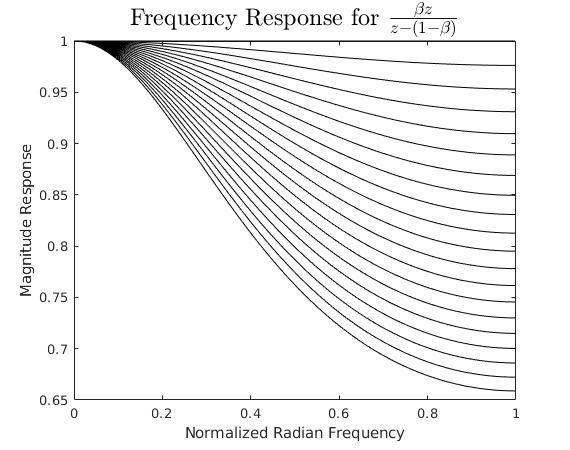
\includegraphics[width=0.8\textwidth]{freqz.png}
    \caption{Frequency response for several moving average exponential filters.  Lower lines are associated with lower values of $\beta$.}
    \label{fig:freqz}
\end{figure}

\subsection{Automatic Differentiation}\label{sec:autodiff}
In all of the previous training algorithms, computation of the gradient of the loss, $\nabla l(w,x,y)$ has been ignored.  This section briefly discuss automatic differentiation, a powerful dynamic programming algorithm for computing the gradient of an arbitrary differentiable function.

Consider some function which depends on multiple variables.  In computing the function, it will likely be expressed as the compositions of other functions.  An example function taken from \cite{ab15} is given below.
\begin{align}\label{eq:autodiff}
f(x_1,x_2) = \log(x_1) + x_1\times x_2 - \sin(x_2)
\end{align}
Equation \ref{eq:autodiff} is a composition of $\log$, $\times$, $\sin$, $+$, and $-$.  This composition can be captured in the form of a graph, as seen in figure \ref{fig:graph}.  Starting at the output and working backwards, one can compute the output of the previous required computation.  Automatic differentiation works in much the same way that a normal computation is performed except by applying the chain rule.  For example, in order to compute the derivative with respect to $x_1$ at node $v_7$, representing the function $[\log(x_1) + x_1\times x_2] - [\sin(x_1)]$, compute $D_{x_1}[\log(x_1) + x_1\times x_2] - D_{x_1}[\sin(x_1)]$.  In order to find the two component values, look at the nodes associated with those functions where the derivative will either already be computed, or where one will compute the derivative by climbing up the graph the same as in the previous step.  Applying this algorithm for all inputs yields the gradient.

\begin{figure}
    \centering
    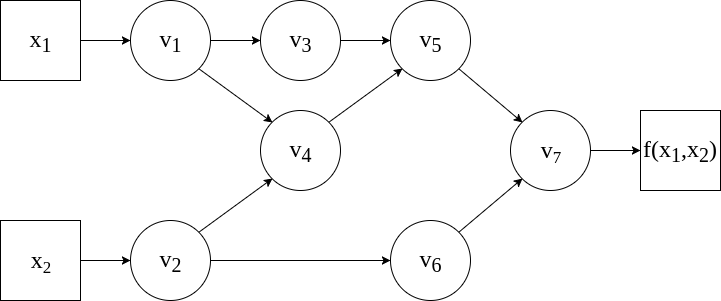
\includegraphics[width=0.8\textwidth]{graph.png}
    \caption{Graph reproduced from \cite{ab15}.  Each node represents a function of the incoming nodes.}
    \label{fig:graph}
\end{figure}

\section{Recurrent Neural Networks}\label{sec:rnn}
Recurrent neural networks are a subset of neural networks which have a key distinction from multilayer perceptrons: they can be applied to data of arbitrary length.  To give more detail we introduce some notation.  Let the set of all n-dimensional vector sequences (finite or otherwise) be given by
\begin{align}
S_n = \{s:Z \rightarrow \mathbb{R}^n; \text{ } \forall Z\subseteq\mathbb{Z}^+\}
\end{align}
While a multilayer perceptron is a function $f:\mathbb{R}^n\rightarrow \mathbb{R}^m$, a recurrent neural network is a function $R: S_n \rightarrow S_m$.

\subsection{Overview}

Of course, the multilayer perceptron could be extended match this if one windows the sequence, compute the output, and then slide the input window.  What truly separates RNNs from MLPs is the fact that an RNN's output depends on its ``state'' at previous time steps.  In particular, denoting the input sequence as $x = (x_1,x_2,\dots,x_k)$ then the states at time steps $1,\dots,k$ are given by equations \ref{eq:rnn_st_start}-\ref{eq:rnn_st_end}.

\begin{align}\label{eq:rnn_st_start}
S_1 &= s(x_1,S_0)\\
S_2 &= s(x_2,s(x_1,S_0))\\
S_3 &= s(x_3,s(x_2,s(x_1,S_0)))\\ \nonumber
&\vdots\\
S_k &= r(x_k,S_{k-1})\label{eq:rnn_st_end}
\end{align}
And the outputs are given by equations \ref{eq:rnn_out_start}-\ref{eq:rnn_out_end}
\begin{align}\label{eq:rnn_out_start}
R_1 &= r(x_1,S_1)\\
R_2 &= r(x_2,r(x_1,S_1))\\
R_3 &= r(x_3,r(x_2,r(x_1,S_1)))\\ \nonumber
&\vdots\\
R_k &= r(x_k,S_{k})\label{eq:rnn_out_end}
\end{align}
If the output sequence is finite, the output of the RNN is the sequence $R(x) = (R_1,R_2,\dots,R_k)$, else it is given by $R(x) = (R_1,R_2,R_3,\dots)$.  The function $s:\R^n \times \R^p \rightarrow \R^p$ is called the state transition function, and the function $r:\R^n \times \R^p \rightarrow \R^p$ is called the output function.  It is assumed that $S_0$ is some arbitrary fixed value (usually zero), called the initial state.  Note that this framework is all very similar to the state-space model, ubiquitous in control theory, except that nonlinearity is allowed in this case.

We can see that the adapted version of the MLP would not be able to represent functions which depend on inputs from time steps farther apart than the length of the window.  In this regard, MLPs are to RNNs as FIR filters are to IIR filters.  Unfortunately because of the non-linearities introduced in RNNs, there is no simple method of analyzing stability, and so training of RNNs has proved difficult throughout their history.  Recent advancements like the long short-term memory unit and dropout have made the training of large RNNs possible.

\subsection{Early Networks}
Some of the first known RNNs, now known as ``simple recurrent networks'' are the Elman \cite{je90} and Jordan \cite{mj86} networks.  The Elman update equations are given by the following equations:
\begin{align}
S_k &= \sigma_S(W_Sx_k+U_SS_{k-1}+b_S\label{eq:elman_s})\\
R_k &= \sigma_R(W_RS_k+b_R)\label{eq:elman_y}
\end{align}
while the Jordan update equations are given by the equations:
\begin{align}
S_k &= \sigma_S(W_Sx_k+U_R R_{k-1}+b_S) \label{eq:newj_s} \\
R_k &= \sigma_R(W_R S_k + b_R) \label{eq:newj_y}
\end{align}
The Elman equations are already in a form consistent with the given framework.  Substituting the second Jordan equation into the first yields the following:
\begin{align}
S_k &= \sigma_S(W_Sx_k+U_R \sigma_R(W_R S_{k-1} + b_R)+b_S)\label{eq:jordan_s}\\
R_k &= \sigma_R(W_R S_k + b_R) \label{eq:jordan_y}
\end{align}
The functions $\sigma_S$ and $\sigma_R$ are sigmoidal activation functions.  The parameters $W_S$,$W_R$, and $U_R$ are matrices, $b_S$ and $b_R$ are bias vectors.

A result analogous to the universal approximation theorem was proved in \cite{hs91}.  Given mild conditions on $r$ and $s$, similar to those of the universal approximation theorem, a recurrent neural net of sufficiently large size is capable of simulating a universal Turing machine.  This means that even a simple RNN (like a Jordan or Elman network) could compute any function, or perform any algorithm that can be performed by a regular computer.  Of course just as with the universal approximation theorem, this says nothing about what is required to train such a network, how many resources it would require, or how efficiently it would operate.

\subsection{Long Short-Term Memory}
Consider computing the derivative of the output of a recurrent neural network with respect to one of its feedback weights, $w$.  By the chain rule:
\begin{align}\label{eq:rnn_deriv}
\frac{d}{dw}R_k(w,x_k,S_k) &= r'(w,x_k,S_k)\times s'(w,x_{k-1},S_{k-1})\times \nonumber
\\&s_{k-1}'(w,x_{k-2},S_{k-2})\times \dots
\times s'(w,x_2,S_1)\times s'(w,x_1,S_0)\\
&= R_k'(x_k,S_k)\prod_{i=1}^k s'(x_i,S_{i-1})
\end{align}
The log derivative is given by
\begin{align}
log(R_k'(x_k,S_k)) + \sum_{i=1}^k \log(s'(x_i,S_{i-1}))
\end{align}
Although it is hard to formally say anything about this value, intuitively since values are being accumulated over time, the log derivative acts as an unstable system.  If the value goes to some very negative number, then the derivative will become extremely small.  On the other hand if the value goes to some very large number, the derivative will become extremely large.  These issues are known as the problems of vanishing and exploding gradients respectively.

The driving cause for exploding or vanishing gradient is that when the state transitions from one time step to another, it is multiplied by some matrix.  The chain rule causes this matrix to be multiplied by itself repeatedly in the derivative calculation which results in either exponential blow up or decay.  The only way to maintain a relatively constant value is for that matrix to be identity, which is exactly the idea behind the long short-term memory (LSTM) unit. \cite{sh97} The update equations for the original LSTM RNN are given by the following:
\begin{align}\label{eq:lstm_start}
i_k &= \sigma_i(W_ix_k + U_iR_{k-1} + b_i)\\
o_k &= \sigma_o(W_ox_k + U_oR_{k-1} + b_o)\\
c_k &= \sigma_c(W_cx_k + U_cR_{k-1} + b_c)\\
S_k &= S_{k-1} + i_k \circ c_k\\
R_k &= \sigma_R(S_k) \circ o_k\label{eq:lstm_end}
\end{align}
Where $\circ$ represents Hadamard (entry-wise) multiplication.

It is easy to see that these equations satisfy the update equations of a standard RNN, as defined.  The direct ``connection'' between $S_k$ and $S_{k-1}$ helps mitigate the issue of vanishing or exploding gradient.  It is important that $i_k$ and $c_k$ can have different signs so that the state is not stuck accumulating in one direction.  For this reason, $\sigma_i$ is usually $\tanh$ while $\sigma_o$ is usually the logistic function.

The model was later extended by \cite{fg00} with what they called a forget gate.  The forget gate, described by the new update equations \ref{eq:forget_1}-\ref{eq:forget_2}, allows the network to essentially discard information in the state and start again.
\begin{align}
f_k &= \sigma_f(W_fx_k + U_fR_{k-1} + b_f)\label{eq:forget_1}\\
S_k &= S_{k-1}\circ f_k + i_k \circ c_k\label{eq:forget_2}
\end{align}

The same group responsible for the invention of forget gates also invented the peephole LSTM. \cite{fg00_2} In this modification of the forget gated LSTM, all instances where the output of the neural network is fed back are replaced with the internal state instead.  For example equation \ref{eq:lstm_start} becomes 
\begin{align}\label{eq:peephole}
i_k = \sigma_i(W_ix_k + U_iS_{k-1})
\end{align}
and so on.

\subsection{Training RNN's}\label{sec:rnn_training}
Recurrent neural networks are trained in much the same way that a standard neural network is trained with one key complication, the input is potentially unbounded.  This means that the number of computations is potentially unbounded and so there is no single graph representing the network.  To solve this issue in computing gradients, the neural network is \emph{unfolded} for some finite amount of time steps.  Any input which goes past the maximum time step is discarded in the computation.

Dropout is a regularization method that can be used to avoid overfitting when training neural networks.  It as applicable to a wide range of neural net models, though its application to recurrent neural networks is slightly more complex.  Essentially, dropout randomly zeros out certain values in the neural net at every time step.  Dropout can be applied at the input, output, or internal state of an LSTM cell.  It was found that applying dropout to state variables led to poor performance, while applying dropout to the output of a cell led to increased performance. \cite{wz14} This type of RNN regularization simply means changing equation \ref{eq:lstm_end} to:
\begin{align}
R_k &= D(\sigma_R(S_k) \circ o_k)
\end{align}
where $D$ zeros random elements of the vector according to independently and identically distributed Bernoulli distributions.


